\documentclass[12pt]{article}

\usepackage{titlesec}
\usepackage{graphicx}

\graphicspath{ {./img/} }
\titleformat{\section}
{\huge\bfseries}
{}
{0em}
{}[\titlerule]

\begin{document}
\title{General Notes on OpenCV and Computer Vision}
\author{}
\date{}
\maketitle


\section{General Concepts}
Before we go into commands specific to OpenCV; we should first understand a little about how image processing works.
\subsection*{HSV Values}
HSV Values are a set of values that represent colors; think RGB values, but instead of Red, Green, and Blue representing the color, it is Hue, Saturation, and Value. But just what do those values mean? Well, let's take a look.
\subsubsection*{Hue}
Hue represents the color portion of an HSV model. These values extend from 0 to 360.

% Format to make fit on same page?
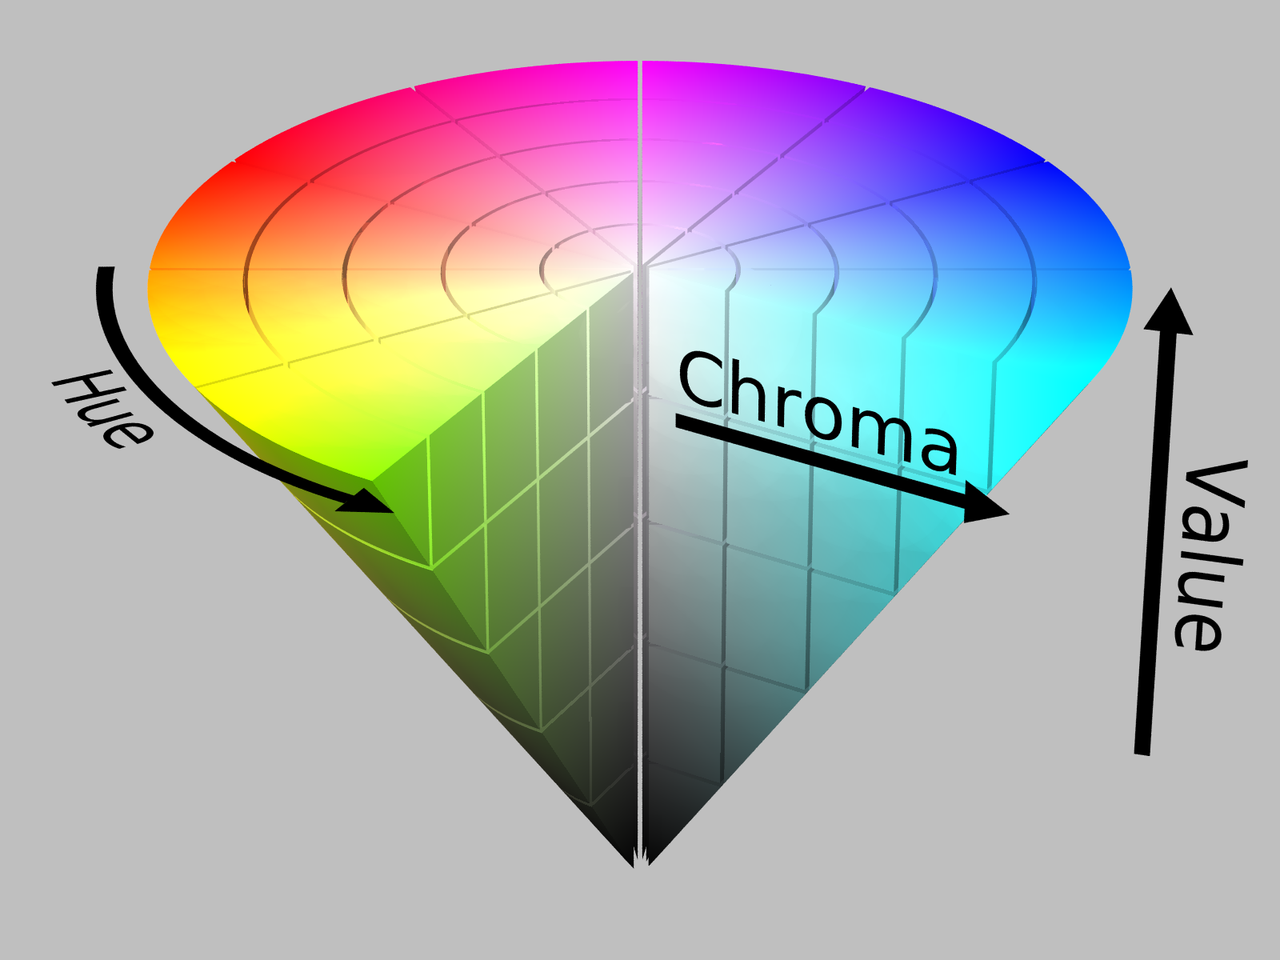
\includegraphics[width=\textwidth]{HSVcolormodel}

\section{Commands}
OpenCV has a variety of commands to increase accuracy of object detection in images. Let's take a look at some and understand how each can improve object detection!
\subsection*{Blurring}
Blurring images can be rather resource intensive, but it is also a great way to reduce noise from an image and get better accuracy when trying to isolate individual objects. Blurs should be applied sparingly and only when necessary given how taxing they can be.
\subsubsection*{Types of Blurs}
Placeholder text
\subsection*{Erosion and Dilation}
Here we will take a look at two important operators for slimming down noise in an image based on the colors of the pixels themselves.
\subsubsection*{Erosion}
Eroding an image will get rid of pixels that are lighter in value by averaging out a certain are (kernel) of pixels.
\subsubsection*{Dilation}
Dilating an image does something fairly similar to eroding one, but instead it will get rid of pixels darker in value.

\end{document}
